\documentclass[border=1pt]{standalone}
\usepackage{tikz}

%Some nicer color definitions
%\definecolor{crimsonred}{RGB}{153,0,0}		% Neurtal red, good for dark or light bg
%\definecolor{darkcharcoal}{RGB}{25,25,25}		% Darker gray
%\definecolor{charcoal}{RGB}{51,51,51}		% Darker gray
%\definecolor{ash}{RGB}{100,100,100}			% medium gray
%\definecolor{paleblue}{RGB}{0,102,102}		% More of an `ocean' color
%\definecolor{clepts}{RGB}{51,153,0}	% A more neutral green
\definecolor{paleale}{RGB}{204,204,102}		% Only for dark BG
%\definecolor{lager}{RGB}{140,110,10}		% Use instead of pale ale for white BG
%\definecolor{cquarks}{RGB}{90,0,120}			% A more neutral purple
%\definecolor{jeans}{RGB}{20,30,150}			% A more neutral blue
%\definecolor{Alert}{RGB}{51,153,0}	

\definecolor{clepts}{RGB}{51,153,0}	% A more neutral green
\definecolor{cquarks}{RGB}{90,0,120}			% A more neutral purple
\definecolor{cbosons}{RGB}{153,0,0}		% Neurtal red, good for dark or light bg


\newcommand{\leg}[4]{\resizebox{1cm}{!}{\begin{tabular}{ccc}
 & #1 &  \\ 
 &  & #2 \\ 
 &  & #3 \\
 & #4 &  
\end{tabular}
}
}

\begin{document}
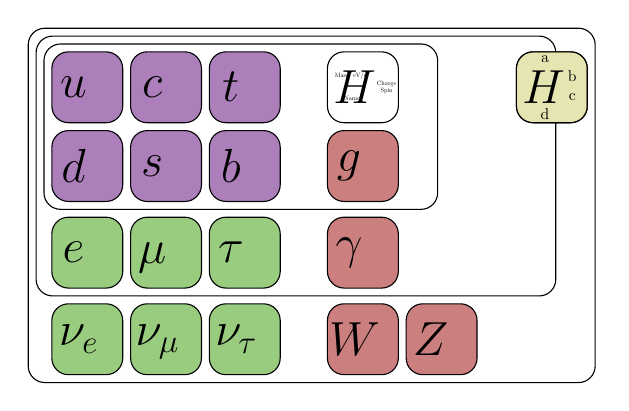
\begin{tikzpicture}[scale=1]


% frame
\draw[rounded corners=6,fill opacity=0] (-0.2,0.2) rectangle (7,-4-0.3);
\draw[rounded corners=6,fill opacity=0] (-0.1,0.1) rectangle (6.5,-3-0.2);
\draw[rounded corners=6,fill opacity=0] (-0.0,0.0) rectangle (5,-2-0.1);

% magenta squares
\draw[rounded corners=6,fill=cquarks,fill opacity=0.5] (0.1,-0.1) rectangle (1,-1) node[pos=0.5,opacity=1,xshift=-5,yshift=0] {\LARGE $u$};
\draw[rounded corners=6,fill=cquarks,fill opacity=0.5] (1+0.1,-0.1) rectangle (1+1,-1)node[pos=0.5,opacity=1,xshift=-5,yshift=0] {\LARGE $c$};
\draw[rounded corners=6,fill=cquarks,fill opacity=0.5] (2+0.1,-0.1) rectangle (2+1,-1)node[pos=0.5,opacity=1,xshift=-5] {\LARGE $t$};
\draw[rounded corners=6,fill=cquarks,fill opacity=0.5] (0.1,-0.1-1) rectangle (1,-1-1)node[pos=0.5,opacity=1,xshift=-5] {\LARGE $d$};
\draw[rounded corners=6,fill=cquarks,fill opacity=0.5] (1+0.1,-0.1-1) rectangle (1+1,-1-1)node[pos=0.5,opacity=1,xshift=-5,yshift=0] {\LARGE $s$};
\draw[rounded corners=6,fill=cquarks,fill opacity=0.5] (2+0.1,-0.1-1) rectangle (2+1,-1-1)node[pos=0.5,opacity=1,xshift=-5] {\LARGE $b$};


% green squares
\draw[rounded corners=6,fill=clepts,fill opacity=0.5] (0.1,-0.2-2) rectangle (1,-1-2-0.1) node[pos=0.5,opacity=1,xshift=-5,yshift=0] {\LARGE $e$};
\draw[rounded corners=6,fill=clepts,fill opacity=0.5] (1+0.1,-0.2-2) rectangle (1+1,-1-2-0.1) node[pos=0.5,opacity=1,xshift=-5,yshift=-2] {\LARGE $\mu$};
\draw[rounded corners=6,fill=clepts,fill opacity=0.5] (2+0.1,-0.2-2) rectangle (2+1,-1-2-0.1) node[pos=0.5,opacity=1,xshift=-5,yshift=0] {\LARGE $\tau$};
\draw[rounded corners=6,fill=clepts,fill opacity=0.5] (0.1,-0.3-3) rectangle (1,-1-3-0.2) node[pos=0.5,opacity=1,xshift=-3,yshift=0] {\LARGE $\nu_e$};
\draw[rounded corners=6,fill=clepts,fill opacity=0.5] (1+0.1,-0.3-3) rectangle (1+1,-1-3-0.2) node[pos=0.5,opacity=1,xshift=-3,yshift=-1] {\LARGE $\nu_\mu$};
\draw[rounded corners=6,fill=clepts,fill opacity=0.5] (2+0.1,-0.3-3) rectangle (2+1,-1-3-0.2) node[pos=0.5,opacity=1,xshift=-3,yshift=0] {\LARGE $\nu_\tau$};

% other squares
\draw[rounded corners=6,fill opacity=0] (3.5 + 0.1, -0.1) rectangle (3.5 + 1, -1) node[pos=0.5,opacity=1,xshift=-3,yshift=0] {\LARGE $H$}  node[pos=0.5,opacity=1] {\leg{Mass: $\mathrm{eV}/c^2$}{Charge}{Spin}{Name}};
\draw[rounded corners=6,fill=cbosons,fill opacity=0.5] (3.5 + 0.1, -1 - 0.1) rectangle (3.5 + 1, -2) node[pos=0.5,opacity=1,xshift=-5,yshift=0] {\LARGE $g$};
\draw[rounded corners=6,fill=cbosons,fill opacity=0.5] (3.5 + 0.1, -2 - 0.2) rectangle (3.5 + 1, -3 - 0.1) node[pos=0.5,opacity=1,xshift=-5,yshift=0] {\LARGE $\gamma$};
\draw[rounded corners=6,fill=cbosons,fill opacity=0.5] (3.5 + 0.1, -3 - 0.3) rectangle (3.5 + 1, -4 - 0.2) node[pos=0.5,opacity=1,xshift=-3,yshift=0] {\LARGE $W$};
\draw[rounded corners=6,fill=cbosons,fill opacity=0.5] (3.5 + 1 + 0.1, -3 - 0.3) rectangle (3.5 + 2, -4 - 0.2) node[pos=0.5,opacity=1,xshift=-4,yshift=0] {\LARGE $Z$};
\draw[rounded corners=6,fill=white,fill opacity=1] (4.9 + 1 + 0.1, -0.1) rectangle (4.9 + 2, -1);
\draw[rounded corners=6,fill=paleale,fill opacity=0.5] (4.9 + 1 + 0.1, -0.1) rectangle (4.9 + 2, -1) node[pos=0.5,opacity=1,xshift=-3,yshift=0] {\LARGE $H$} node[pos=0.5,opacity=1] {\leg{a}{b}{c}{d}};









\end{tikzpicture}
\end{document}